\documentclass[a4paper,10pt]{article}

\usepackage[boxruled,vlined,english]{algorithm2e}
\usepackage[francais,english]{babel}
\usepackage[utf8x]{inputenc}
\usepackage[T1]{fontenc}
\usepackage{graphicx}
\usepackage{hyperref}
\usepackage{latexsym}
\usepackage{setspace}
\usepackage{amsmath}
\usepackage{amssymb}
\usepackage{bookman}
\usepackage{amsthm}
\usepackage{amscd}
\usepackage{color}
\usepackage{calc}

\setlength{\voffset}{-3.75cm}
\setlength{\hoffset}{-2.6cm}
\setlength{\oddsidemargin}{2.75cm}
\setlength{\topmargin}{2in}
\setlength{\headheight}{0in}
\setlength{\headsep}{0in}
\setlength{\topskip}{0in}
\setlength{\parindent}{0cm}
\setlength{\parskip}{1ex plus0.4ex minus0.2ex}
\setlength{\textwidth}{17cm}
\setlength{\textheight}{22cm}
\renewcommand{\baselinestretch}{1.5}
\flushbottom
\setcounter{page}{1}
\setcounter{tocdepth}{2}

\SetKw{Edb}{Side effect}
\SetKw{Et}{and}
\SetKw{Ou}{or}
\SetKw{De}{from}
\SetKw{A}{to}
\SetKw{Par}{by}
\SetKwBlock{Debut}{Begin}{End}
\SetKwIF{Si}{SinonSi}{Sinon}{If}{then}{Else if}{Else}{EndIf}
\SetKwFor{Pour}{For}{do}{EndFor}
\SetKwFor{PourTout}{For all}{do}{EndFor}
\SetKwFor{TantQue}{While}{do}{EndWhile}
\SetKw{Retour}{Return}

\newcommand{\guill}[1]{``#1''}
\newcommand{\bigO}[1]{\mathcal O\left( #1 \right)}
\newcommand{\bigOmega}[1]{\Omega\left( #1 \right)}
\newcommand{\bigTheta}[1]{\Theta\left( #1 \right)}




% ??? Faire une Titlepage un peu plus jolie...
\title{ \Large Internship report \\ \LARGE Computational analysis of jazz chord sequences}

\author{\normalsize Romain \textsc{Versaevel}, M1 Informatique Fondamentale, ENS de Lyon\\
\normalsize Tutored by David \textsc{Meredith}, Associate professor at Aalborg University,\\
\normalsize leader of the Music Informatics and Cognition group\\}

\date{\today}

\begin{document}

\maketitle

\begin{abstract}
\noindent
I report here the results of my work at Aalborg University during the summer 2015. My main task was to provide an analysis of a dataset of chord sequences from jazz songs.

\noindent
For this, I performed two kinds of analysis, one using the LZ77 compressing algorithm and one computing \emph{diagonal patterns}; the performances of these algorithms were improved by introducing compression with loss through the use of \emph{similarity measures} between chords. The obtained analysis is successful; it validates the method I used and shows room for further research; its main result is to suggest that jazz chord sequences structure should rather be seen as a whole than linearly.

\noindent
The algorithms, their results, as well as a short introduction to Computer music can be found in the report.
\end{abstract}

\newpage
\tableofcontents
\newpage


\section{Introduction}

This report presents the twelve-week internship I did as part of my Master 1 of Computer Sciences at ENS Lyon. This internship took place at Aalborg University, Denmark, from May 25th 2015 to August 14th, in the Department of Architecture, Design and Media Technology. I was supervised by Pr. David Meredith, who is Associate Professor there and specializes in Computer music.

During this internship I mainly worked on Computational music analysis, and especially the analysis of a dataset of chord sequences from popular jazz songs.

The report has three main sections.
The first one consists in an introduction to the research field, \emph{Computer music}.
The second describes my work on the jazz chords dataset, consisting in two different ways of compressing it, and the obtained results.
Finally possible improvements and unrelated work I did are shown in a third section.

An appendix with more details (additional definitions, examples of the algorithms execution, exhaustive numerical results\dots) can be found on \href{https://github.com/Rometach/aalborg/blob/master/Rapport/appendix.pdf}{the GitHub repository} I used.



\section{Computer music}

This section briefly introduces the area of \emph{Computer music}. It aims at giving to the non-expert reader a glimpse of the context and motivation of my work. I present first the general field, and then the more precise domain of Computational music analysis.


\subsection{Short presentation, history, research areas}

The term \emph{Computer music} simply describes any activity that implies both music and computing tools.

Music and mathematics have been linked from the origins; the basis of western music was developed by the Pythagoreans in the 5th century BCE; the French composer Jean-Philippe Rameau used mathematical tools to theorise harmony in the 18th century, in \cite{rameau} for example. Sound is a physical vibration, and has mathematical properties; and western music is structured at every level by numbers. Hence, the birth and development of Computer music naturally quickly followed the one of computers. The progress of computation offered new tools to music musicology; simultaneously, the all-analogue world of audio became almost all-numerical.

Computer music is therefore a young science (the first pieces composed with the help of computers appeared in the late 50s), based on a very ancient one. In Computer sciences, it is related to \emph{Computational linguistics}; it can be close to Cognitive sciences and often uses techniques from Machine learning.

Its research areas are numerous and diversified. One can deal with audio data (recordings, live performance\dots) or symbolic one (MIDI scores\dots); one can study existing pieces or aim at producing new ones; one can improve the laypersons' or the professional musicians' experience. Here is a non-exhaustive list of research areas being part of Computer music:

\begin{itemize}
\itemsep0em 
\item[$\triangleright$] automated composition or orchestration;
\item[$\triangleright$] automated live improvisation;
\item[$\triangleright$] computational music analysis;
\item[$\triangleright$] music representation;
\item[$\triangleright$] signal processing\dots
\end{itemize}

\subsection{Computational music analysis}

Why analysing music with computers? As stated above, because computers provide researchers brand new ways of studying music. My analysis hereafter, for example, requires too many computations for a human being, and on the other hand no peculiar musical skills. And what kind of \emph{analysis} can computers achieve? Anything that can help the work of musicologists will be called an analysis; the most common ways to do so are pattern discovery (as I will do here) and segmentation.

As for the general case, analysis can be of audio material or of symbolic representation (or both); its goal can be to acquire knowledge or the ability of creating new pieces (or both). The analysis I give here focuses only on symbolic data and it purpose is rather a learning one.

At the beginning of my internship, my work was mainly bibliographical, to become more familiar with the diversity of existing techniques for Computational music analysis. A reader who would like to do the same may want to read papers using probabilistic grammars (\cite{goldabdallah}), Markov chains and $n$-grams (\cite{markov1}, \cite{markov2}, \cite{markov3}), geometrical patterns (\cite{cosiatec}), or tries (prefix trees) (\cite{patminr}).


%\subsection{Several techniques}
%
%\subsubsection{Schenker}
%\subsubsection{http://webprojects.eecs.qmul.ac.uk/marcusp/papers/PearceWiggins2012.pdf}
%\subsubsection{http://axon.cs.byu.edu/~dan/673/papers/pachet.pdf}
%\subsubsection{http://citeseerx.ist.psu.edu/viewdoc/download?doi=10.1.1.3.5364&rep=rep1&type=pdf}
%\subsubsection{COSIATEC}
%\subsubsection{PatMinr}


\newpage
\section{Analysing jazz chord sequences}

This section presents my concrete work and contribution. After a presentation of the data motiva\-ting this work, jazz lead sheets, I introduce the main tools I used, chord similarity measures and compression algorithms, and finally I give and discuss the results obtained.

\subsection{Motivation}

The main motivation of my work was a dataset of jazz lead sheets, provided by \href{http://www.csl.sony.fr/music.php}{Sony CSL}. Before going into more details, I have to introduce basic musical definitions so as to make myself more understandable. I try here to give enough explanations for anyone to understand what I will deal with, but also clues for a more interested reader who would like to glimpse mathematical models of music.

In jazz music, songs are displayed in the form of \emph{lead sheets}, scores giving the base melody with extra indications of chords. An extract of a lead sheet for \emph{What a wonderful world} can by seen on figure \ref{waww}; the sung melody is written on a staff and the chords are visible in handwritten font.

\begin{figure}[h!]
\centering
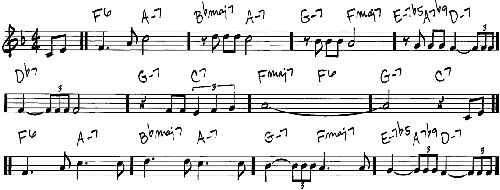
\includegraphics[width=10cm]{images/waww.jpg}
\caption{Lead sheet with the beginning of Louis Armstrong's \emph{What a wonderful world}\label{waww}}
\end{figure}

A \emph{chord} is a set of (at least three) notes; in this context, they are used to give the current mood of the piece, and jazz musicians can improvise the accompaniment of the melody with the notes of the chord. Chords are represented\footnote{~~There are several ways of representing chords; this representation, the \emph{tabular notation}, is the most common in popular music (jazz, pop, rock\dots). But for instance, superposed notes on a classical music staff would also represent a chord.} 
by a letter from $A$ to $G$\footnote{~~French equivalent: from \emph{la} to \emph{sol}.} 
with a possible \emph{accidental} ($\#$ for \emph{sharp}, $\flat$ for \emph{flat}, or nothing), representing the \emph{root note}, and a textual information giving the other notes relatively to the root note. For example, if we consider the $C\#m7$ chord (\guill{$C$ sharp minor seventh}), the notes will be the root note $C\#$, its \emph{minor third} $E$, its \emph{fifth} $G\#$ and its \emph{minor seventh} $B$. In jazz there are 313 possible such textual informations
\footnote{~~Actually, one could theoretically form different 56320 chords for a given root note; those 313 correspond to the \guill{harmonious} combinations, which is a subjective notion and thus depends on the music genre.}.

The dataset I worked on contains the lead sheets of 30 jazz pieces by famous artists like Louis Armstrong, Billie Holiday, Charlie Parker\dots~Some files describe the melodies as a sequence of notes (with pitch, onset and duration informations) and other contain the sequences of chords (sometimes with onset and duration informations). I did focus on the chord sequences with no timing information (as if for instance there was exactly one chord per bar). So, my data basically looked like:

\begin{equation*}
\text{\textbf{A Child Is Born:} } B\flat M7;~E\flat m;~B\flat M7;~E\flat m6;~B\flat M9;~E\flat m;~A~halfdim7;~D 7\#9\dots
\end{equation*}

I equally worked on the chord sequences of each song and on the concatenation of all the available sequences. This concatenation does not really make sense as a unique piece, but it is useful to do so in order to have an overview of all the corpus. On what follows, I will concentrate on the results of my algorithms on this concatenation.

So, the motivation of my work was to provide an analysis of this data. The purpose of such an analysis is to gain knowledge about jazz and chord sequences, understanding it better, and also in a second time to use this knowledge to be able to compose similar music that would fit in the corpus.



\subsection{Chord similarities}

This section introduces the concept of chord similarity measures, central in my analysis, and defines some measures from the state-of-the-art that I used.

\subsubsection{Introduction}

There are only 12 possible root notes because two notes separated by an \emph{octave} (concretely, whose frequencies ratio is a power of two) sound likewise, and are thus called the same: $C$ refers to low-pitched as well as to high-pitched sounds. The 12 notes correspond to a division of the octave into twelve equivalent \emph{semitones}; this is called the \guill{well-tempered} scale. 
So, as shown on figure \ref{keyboard}, the keyboard can be mapped to the cyclic group $\mathbb{Z}/12\mathbb{Z}$, and the notes to integers from $0$ to $11$.

\begin{figure}[h!]
\centering
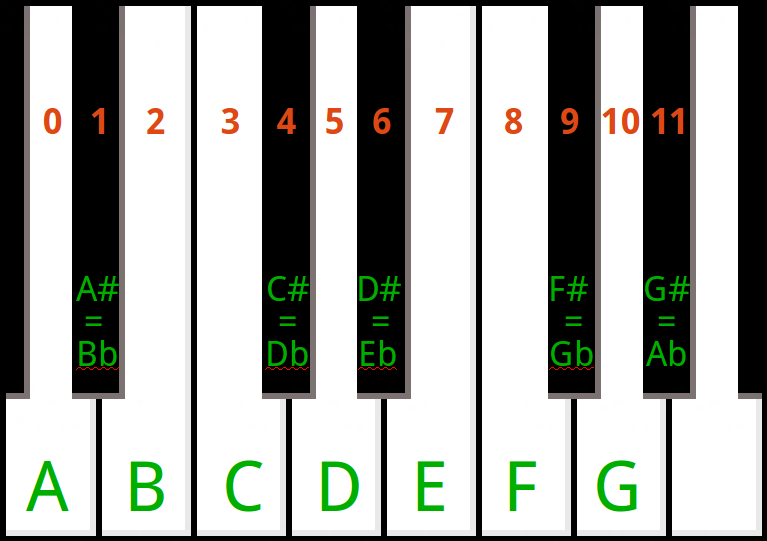
\includegraphics[width=5
cm]{images/keyboard+.jpg}
\caption{A keyboard with notes names and their equivalent in $\mathbb{Z}/12\mathbb{Z}$\label{keyboard}}
\end{figure}

Then chords can be seen as subsets of $\mathbb{Z}/12\mathbb{Z}$. For instance, the previously seen $C\#m7$ chord would be mapped to the set $\{4;7;11;2\}$ (the order does not matter). Moreover the harmonic content in the chord name (here, \guill{$m7$}) can be seen as the vector and the root note (\guill{$C\#$}) as a starting point. Chords with same labels but different root notes are then the same by translation: $C\#m7$ corresponds to $\{4;7;11;2\}$ and $D\#m7$ to $\{5;8;12;3\}=\{4;7;11;2\}+\{1;1;1;1\}$.

It is hence possible to define mathematically distances between chord. However, such a distance much be chosen carefully to be relevant. Canonical distances do not necessarily mirror what is heard. With the $L_1$ distance (\guill{taxicab metric}) on chords of three notes, the chords $C=\{3;7;10\}$ and $Cm=\{3;6;10\}$ would be close since the difference is only of one semitone ($L_1(C,Cm)=1$); but to the ear they sound very different, one being major and the other minor. On the contrary, one would here something common between $C=\{3;7;10\}$ and $Bm=\{2;5;9\}$: they are \guill{inversions} of each other.


\subsubsection{List of used measures}

In all, I used 9 different measures (in addition to the most simple one: equality), some rather elementary, some expressly developed by researchers. Three take as input the two chords to compare, $C_1$ and $C_2$, and return a boolean (\texttt{true} if and only if the chords are similar). All three define equivalence classes. They are:

\begin{itemize}
\itemsep0em 
\item[$\triangleright$] root note equivalence: \texttt{true} iff $C_1$ and $C_2$ have the same root note;
\item[$\triangleright$] translational\footnote{~~\guill{translation} is the mathematical word; musicians would prefer \guill{transposition}.} 
equivalence: \texttt{true} iff $C_1$ and $C_2$ have the same harmonic indication (but possibly different root notes);
\item[$\triangleright$] PCS-Prime equivalence (see \cite{forte}): \texttt{true} iff $C_1$ can be obtained from $C_2$ by a composition of inversions and translations.
\end{itemize}

The six other are distances\footnote{~~I use the word \guill{distance} to emphasize the difference with the first three measures; however all are not distances in a mathematical definition.}: they take as input two chords $C_1$ and $C_2$ and return a positive real number (all are scaled so that their image is $[0,1]$). As I will show in the next part, I did need this value only to determine if two chords are \guill{close} of \guill{different}, so I used them with a threshold as additional input parameter. The measure will then return \texttt{true} if and only if the distance between $C_1$ and $C_2$ is less than the threshold.

They are the F1-score (cardinality of the intersection divided by the sum of the cardinalities, multiplied by two); Eric Isaacson's similarity index, defined in \cite{isaacson}; David Lewin's measure, defined in \cite{lewin}; Robert Morris' measure, defined in \cite{morris}; John Rahn's measure, defined in \cite{rahn}; Richard Teitelbaum's measure, defined in \cite{teitelbaum}.

%\begin{itemize}
%\itemsep0em 
%\item[$\triangleright$] the F1-score (cardinality of the intersection divided by the sum of the cardinalities, multiplied by two);
%\item[$\triangleright$] Isaacson's similarity index, defined in \cite{isaacson};
%\item[$\triangleright$] Lewin's measure, defined in \cite{lewin};
%\item[$\triangleright$] Morris' measure, defined in \cite{morris};
%\item[$\triangleright$] Rahn's measure, defined in \cite{rahn};
%\item[$\triangleright$] Teitelbaum's measure, defined in \cite{teitelbaum}.
%\end{itemize}

The definitions of all these measures can be found in appendix. Here I will only present as an example Isaacson's similarity index. It is a relatively arbitrary choice since, as I will point later, all this measures gave close results, but this one allows me to introduce the interesting notion of interval vector.

Given a set $S\subset\mathcal{P}([0,11])$, its associated \emph{interval vector} is a vector $IV(S)\in\mathbb{N}^6$ such that the $i$-th coordinate of $IV(S)$ is the number of pairs of elements in $S$ whose difference is $i$. In other words, we look at the intervals inside $S$: how many intervals of length $1$, of length $2$, etc. The interval vector is an histogram for these values. 

For instance, for a seventh major chord, whose corresponding set is $\{0;4;7;10\}$, we have $1$ interval of length $2$ (between $0$ and $10$), $2$ of length $3$ ($4$ and $7$, $7$ and $10$), $1$ of length $4$ ($0$ and $4$), $1$ of length 5 ($0$ and $7$) and $1$ of length $6$ ($4$ and $10$). Hence $IV(\{0;4;7;10\})=(0,1,2,1,1,1)$. There are $6$ and not $12$ coordinates because these intervals are not oriented (modulo $12$, going from $1$ to $8$ is the same as going from $8$ to $12+1=13$, and the interval has then a length of $5$).

Isaacson's similarity index is defined as the \emph{standard deviation} function applied to the interval vectors. For chords denoted $X$ and $Y$ having interval vectors $IV_X=(x_1,\dots,x_6)$ and $IV_Y=(y_1,\dots,y_6)$, let us write $D$ the difference vector $((y_1-x_1),\dots,(y_6-x_6))$ and $\bar{D}$ the mean of the $(y_i-x_i)$s. The measure is finally:

\begin{equation*}
\mathfrak{M}_{Isaacson}(X,Y) = \sqrt{\frac{1}{6}\left(\sum_{i=1}^6\left(D_i-\bar{D}\right)^2\right)}
\end{equation*}


\subsection{Compression algorithms}

The words \guill{analysis} and \guill{compression} will be used here with very close meanings. Indeed, compressing a piece means exhibiting its structure, separating the essential from the redundant. Hence, my analysis of the jazz lead sheets dataset will be described in terms of compression, and evaluated as such.

There are two complementary ways to approach computational music analysis
\footnote{~~They are of course also relevant in a wider context.}. 
One sees a piece as a linear sequence of notes (or chords, etc.), as the listener does: he can remember everything he heard but has no way to know what is coming until he actually hears it. The other views the piece from above, completely. Roughly, the first deals with linked lists and the second with arrays. It is the approach of Markov models \emph{versus} the one of formal grammars, Shannon's entropy \emph{versus} Kolmogorov's complexity.

My way of compressing simply describes a sequence of chords through the patterns (repeated sub-sequences) it contains, thus removing the redundancy. I developed it, implemented and tested algorithms for both approaches (linear and global), in order to be able to compare them. For the former, I used the classical algorithm known as LZ77; for the latter, a \guill{diagonal pattern decomposition}. They are presented in this order, after some basic definitions.


\subsubsection{Definitions}

The compressions are evaluated with their \emph{compression factor} and \emph{loss factor}.

The \emph{compression factor} corresponds to the size of the input data divided by the size of the compressed data. It is expected to be as high as possible (and at least greater than $1$). In here, it is considered that the size of a chord is the same as the size of an integer. Indeed, their are $7\cdot4\cdot313=6573$ possible chords, so a chord can be described with $\lceil log_2(6573)\rceil = 13$ bits; and the integer dealt with are lesser than $1469$ (the total number of chords in the database), thus defined by $\lceil log_2(6573)\rceil = 11$ bits. Of course, this definition fits the data I used and a different one could be needed for a different data.

There exist compression algorithms \emph{with} and \emph{without loss}. \emph{Without loss} means that the decompression of the compression is equal to the original sequence, while \emph{with loss} it is not necessarily so. The advantage of a compression with loss is that it can achieve better compression factors. I will define here the \emph{recovery factor} as the number of exact chords in the decompression of the compression of a piece, divided by the length of the piece. It is thus a real number between $0$ and $1$, that we will expect to be as close to $1$ as possible. This definition is rather sensitive; indeed, the loss will result of the use of similarity measures, and the original chords will be replaced during the compression by similar ones. However, the only other way to define would be to use precisely the similarity measure (\guill{the two corresponding chords are different by at most $x$ according to the measure}) but in my eyes not having an external evaluation would mean have too much faith in the measures; moreover one understands well what it is to be equal or different, but has no precise idea of what a difference of $x$ in a given measure could mean.


\subsubsection{Lempel-Ziv 77 (LZ77)}

The LZ77 algorithm, designed by A. Lempel and J. Ziv in 1977, introduced in \cite{lempelziv}, is a very popular compressing algorithm. It takes as input a list of data and outputs a list of triples of the form $(a,b,D)$ meaning \guill{go back $a$ times, copy the next $b$ data, and add $D$}. In the original algorithm, restrained buffer and preview size are given as parameters; however, I chose to let them be unbounded in order to focus on the best possible results. The obtained algorithm is given in \ref{algolz77}.

\begin{algorithm}
\setstretch{1.5}
\caption{LZ77 \label{algolz77}}
\SetKwData{iii}{i} \SetKwData{jjj}{j} \SetKwData{III}{I} \SetKwData{pref}{$\pi$} \SetKwData{aaa}{a} \SetKwData{bbb}{b} \SetKwData{buffer}{buffer} \SetKwData{LLL}{L}
\SetKwFunction{push}{push} \SetKwFunction{pop}{pop} \SetKwFunction{front}{front} \SetKwFunction{size}{size}

\KwIn{Queue of Chords $\III=(C_1, \dots, C_n)$.}
\KwOut{Queue of triples $\LLL=(a_j,b_j,C_{i_j})_j$.}

\Debut {
	\buffer $\leftarrow$ empty queue 

	\TantQue{\III is not empty} {
		\pref $\leftarrow$ longest prefix of \III in $(\buffer\cdot\III)$, beginning in \buffer

		\aaa $\leftarrow$ $\size(\buffer)$ $-$ (beginning index of \pref (in \buffer)) ($0$ if none)

		\bbb $\leftarrow$ length of \pref ($0$ if none)

		\Pour{\jjj \De $1$ \A \bbb} {
			$\buffer.\push(\front(\III))$

			$\III.\pop()$
		}
		$\LLL.\push(\aaa,\bbb,\front(\III))$

		$\buffer.\push(\front(\III))$

		$\III.\pop()$
	}
	\Retour \LLL
}
\end{algorithm}


For a better understanding, a complete example of an execution of the algorithm is given in appendix.

With a computation of the longest prefix in $\bigO{|\texttt{I}|^2}$, the overall complexity is $\bigO{|\texttt{I}|^3}$. There are better evaluations of this complexity but that are not of much interest here; knowing that it is polynomial and that the implementation runs fast is enough.

The LZ77 algorithm performs a compression without loss. I modified it in order to have a compression \emph{with loss}. The modification is very simple: when looking for the longest prefix, the algorithm will not only accept identical sequences, but also sequences that are similar up to a certain point. For a given measure $\mathfrak{M}$ and a threshold $t$ (let us assume that the image of $\mathfrak{M}$ is $[0,1]$ and that higher values correspond to more similar chords), two sequences $S_1$ and $S_2$ of the same length $n$ are considered similar if $\forall i \in [1,n], \mathfrak{M}(S_1[i],S_2[i]) \geq t$.


\subsubsection{Diagonal pattern decomposition}
\label{compressiondiagonal}

My second approach uses \emph{diagonal patterns}. The best way to understand this notion is to visualise it. For a given piece, we write the chord sequence both vertically and horizontally. We can then consider a matrix whose cell $(i,j)$ will correspond to the $i$th and $j$th chords of the input sequence. Let us draw this cell in white if those chords are equal, and in black if they are different. We get a binary matrix on which  we can see the diagonal patterns, which are diagonal sequences of white cells. They correspond to sequence of chords that appear (at least) twice in the input piece, on two different positions. Such a matrix can be seen on figure \ref{diagonals}.

\begin{figure}[h]
\centering
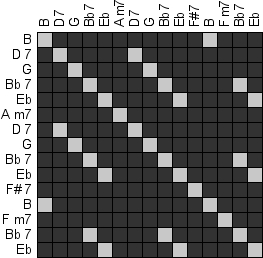
\includegraphics[width=6cm]{images/diagonals1.jpg}\hspace{1cm}
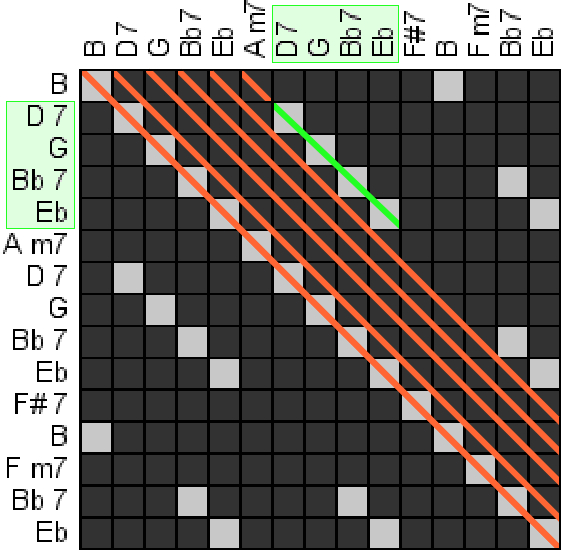
\includegraphics[width=6cm]{images/diagonals2.jpg}
\caption{A binary matrix and the diagonal search for patterns\label{diagonals}}
\end{figure}

A \emph{pattern} will then precisely be a maximal such sequence, along with its occurrences (positions where it occurs). \emph{Maximal} means that we consider only sequences having an occurrence that cannot be extended. Figure \ref{diagonals} shows the diagonal search for patterns and the maximal pattern $D7GB\flat 7E\flat$. $D7G$ is not maximal: every times it occurs it can be extended in the end. On the contrary, $B\flat 7E\flat$, which is included in $D7GB\flat 7E\flat$, is also a maximal pattern, occurring in the very end. In the piece of figure \ref{diagonals}, the diagonal patterns are (by increasing size):

\begin{tabular}{rl}
$\triangleright$ & $B$, on positions 0 and 11; \\
$\triangleright$ & $B\flat 7E\flat$, on positions 4, 8 and 13; \\
$\triangleright$ & $D7GB\flat 7E\flat$, on positions 1 and 6.\\
\end{tabular}

%\begin{itemize}
%\item[$\triangleright$] $B$, on positions 0 and 11;
%\item[$\triangleright$] $B\flat 7E\flat$, on positions 4, 8 and 13;
%\item[$\triangleright$] $D7GB\flat 7E\flat$, on positions 1 and 6.
%\end{itemize}

As for the LZ77, I introduce here similarity measures, which will lead to a compression with loss. Instead of drawing a cell of the matrix in white only if the two corresponding chords are equal, this will be done also if they are similar for a given measure and up to a certain threshold. The matrix has then more white cells, implying more and longer patterns. Figure \ref{loose} shows this transformation (with the F1-score and a threshold of $0.9$).

\begin{figure}
\centering
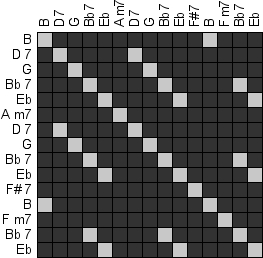
\includegraphics[width=6cm]{images/diagonals1.jpg}\hspace{1cm}
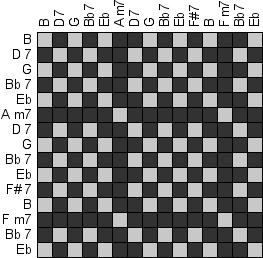
\includegraphics[width=6cm]{images/diagonals3.jpg}
\caption{Binary matrices for the same piece, the second using a similarity measure (F1 score)\label{loose}}
\end{figure}


Once the list of patterns established, the next step is to select a subset of these which is sufficient to describe the whole piece. In order to be sure this will always be possible (which is not the case in our example!), we add a \guill{pattern} for each single chord appearing in the piece (here: $(B;0,11)$, $(D7;1)$, $(G;2)$\dots). This subset should be as \guill{light} as possible, the \emph{weight} of a pattern being the sum of its length and of its number of occurrences. This problem is a \emph{weighted set cover}, which is NP-complete\footnote{~~See \href{https://en.wikipedia.org/wiki/Set\_cover\_problem}{https://en.wikipedia.org/wiki/Set\_cover\_problem} for more explanations on the set cover problem.}. So I implemented two heuristics, and the lighter results of the two will be selected. Briefly, their are both greedy algorithms; one aggregates patterns until covering the whole piece and the other removes as many patterns as possible from the exhaustive list. The pseudo-codes of these are given in the appendix.

For the decompression algorithm, the selected patterns are sorted by increasing number of occurrences and are copied in this order (so, a position that is covered by several patterns can be rewritten several times, and only the last, i.\!e. the corresponding chord of the pattern with most occurrences, will be kept). It is used to compute the \emph{recovery factor}. A pre-treatment is done on the patterns in order to maximize it (to minimize the loss). Indeed, a pattern occurring \emph{similarly} several times can correspond to several different exact sequences, and the recovery factor will depend on the choice of the sequence (which does not impact the compression factor) representing the pattern. For this, I simply compute for every pattern what positions of the reconstruction depend on it, and choose among the possible sequences the one that implies a minimum loss\footnote{~~This greedy algorithm, knowing the decompression scheme, finds obviously the optimal configuration this problem.}.

The complexity of the whole algorithm is $\bigO{|I|^5}$\footnote{~~See appendix for a brief analysis.}. This is quite high. In practice, the number of maximal patterns (which is $\bigO{|I|^2}$ in the worst case) seems to be the most determining factor for the running time. On my complete database (approximately 1500 chords), the execution takes between a few seconds and several minutes.


\subsection{Results}

This sections presents the results obtained by the two compression algorithms, for several measures and several thresholds. I focus here on their interpretation; more exhaustive results can be found in appendix.

\subsubsection*{Comparison between measures}

The $10$ (including equality) different measures I used resulted, of course, in different compressing results. Binary matrices look differently; recovery and compression factors as functions of the thresholds look differently. However, surprisingly, there is a correlation between those two factors, independent from the measure used, as can be seen on figure \ref{rfc}. This validates the use of the F1-score, which in contrary to other measures is not designed especially for music, in this field.

\begin{figure}[h]
\centering
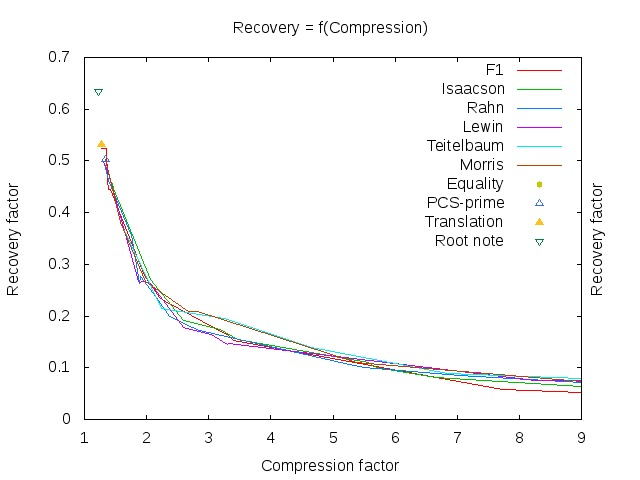
\includegraphics[width=7cm]{images/RfC77.jpg}\hspace{0.5cm}
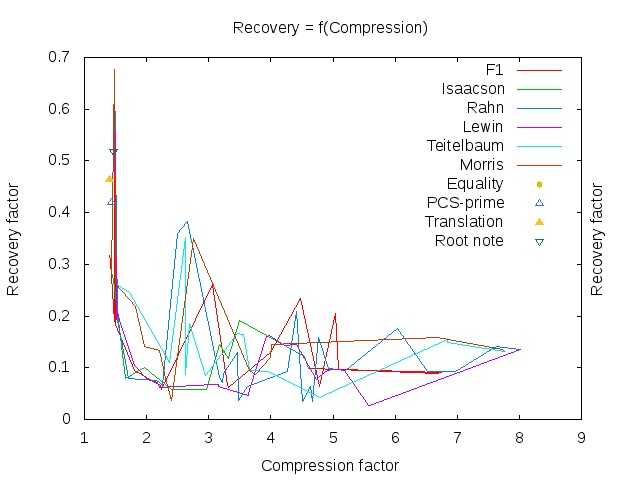
\includegraphics[width=7cm]{images/RfCDiag.jpg}
\caption{Link between recovery and compression factors (left: LZ77, right: diagonal patterns)\label{rfc}}
\end{figure}

In the case of the LZ77 algorithm, the results are really the same. For the diagonal patterns algorithm, some measures are \guill{leading} around several values of compression factors; but it is hard to determine if it comes from the irregularities of the algorithm or really shows a kind of superiority.

As I said before, I use the recovery factor in order to have a way of evaluating exterior to the measures. Nevertheless, differences between them appear if we are confident in their ability to reflect musical closeness between chords. Indeed, in the case of the diagonal patterns algorithm, the best compression factors are not obtained for the same thresholds. All lead to highest compressions for medium thresholds, except for Isaacson's similarity index, on figure \ref{isaacson}. This could be fortuitous, or mean that this precise measure is particularly adapted to the analysis of jazz chords. The best way to find out the truth would be to have the opinion of a skilled musician, who for instance would listen to the original piece and the decompression of the compression.

\begin{figure}[h]
\centering
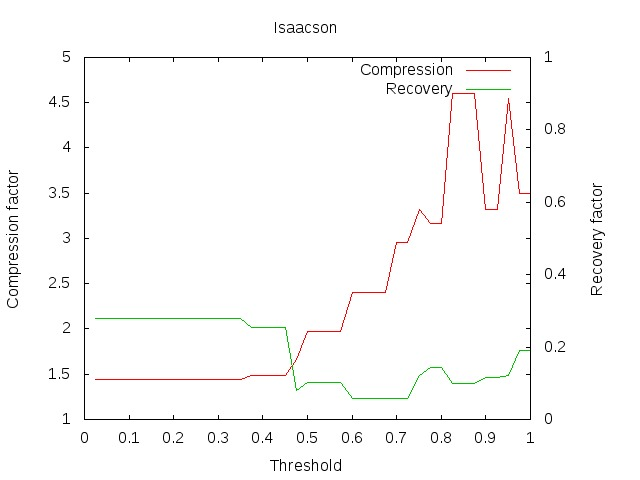
\includegraphics[width=7cm]{images/IsaacsonDiag.jpg}
\caption{Diagonal compression with Isaacson's measure\label{isaacson}}
\end{figure}

\subsubsection*{The interest of similarity measures}

The measures with no thresholds result in relatively low compression factors (and high recovery factors). The gain provided by the use of similarity measures becomes obvious with the ones using thresholds. They make possible a wide range of compression factors. Without them, i.\!e. with the equality, the LZ77 does not even compress: the compression factor is $0.931258<1$ !


\subsubsection*{Comparison between algorithms}

First, one observes on figure \ref{rfc} that the results of the diagonal patterns algorithm are a lot more \guill{chaotic} than the results of the LZ77 algorithm. Those are very regular: the compression factor is almost always a decreasing function (and the recovery factor an increasing function) of the similarity, represented by the threshold.

In my opinion, the main reason for the irregularities in the diagonal patterns algorithm is linked to the approximations made when solving the set cover problem\footnote{~~For the set cover problem without weights, the greedy algorithm similar to one I use performs a $H_n$-approximation, $H_n$ being the $n$-th harmonic number (for $n$ the size of the problem); this is of the order of $\ln(n)$.}.
Moreover, it is not clear like for the LZ77 algorithm that loosening the threshold should improve the compression. For instance, there can be a pattern appearing several times such that, after the loosening, some of its occurrences are extended and some not; we would then have two patterns or more, and the sum of their weights would be greater than the weight of the single pattern.

Despite this, the second important observation is that for the same compression factors, the recovery factor is generally higher (except around $2$) with the diagonal patterns algorithm. This may lead to think that the second paradigm of analysis (the \guill{view from above}, opposed to the \guill{linear} approach) better fits jazz chord sequences\footnote{One should be cautious, of course, since the LZ77 algorithm is not as complex; on the other hand I stated that the diagonal patterns algorithm could be improved.}.



\newpage
\section{Other and further work}

In this section I present ways I foresaw to improve my work, or develop it into new directions, and my (small) contribution to the Lr2Cr8 project. All of this represent a non-negligible part of my work in Aalborg. I focused in this report on my most complete results; here I try do give hints of the rest, general ideas rather than details.


\subsection{Segmentation? Grammatical inference?}

The drawings of binary matrices used for compression (section \ref{compressiondiagonal}), like figure \ref{pretty}, reveals pretty geometrical configurations, symmetries, hence structure. My compression is a way among, I am sure, many others to capture this structure.

\begin{figure}[h]
\centering
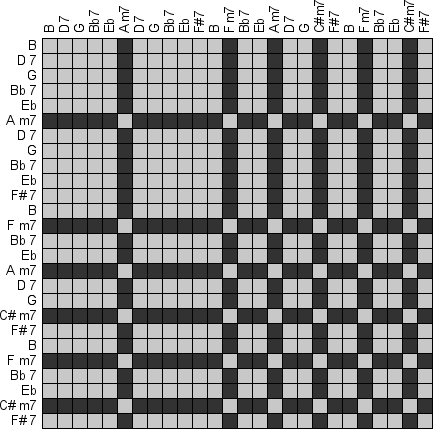
\includegraphics[width=3.5cm]{images/pretty1.jpg}\hspace{0.5cm}
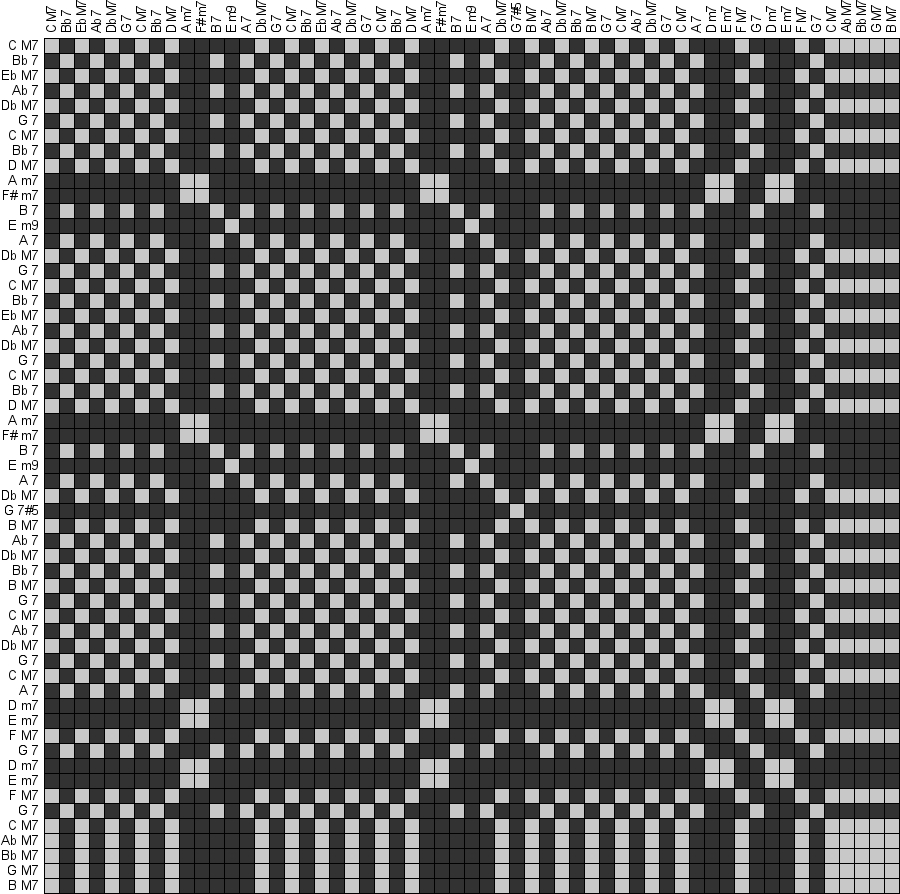
\includegraphics[width=3.5cm]{images/pretty2.jpg}\hspace{0.5cm}
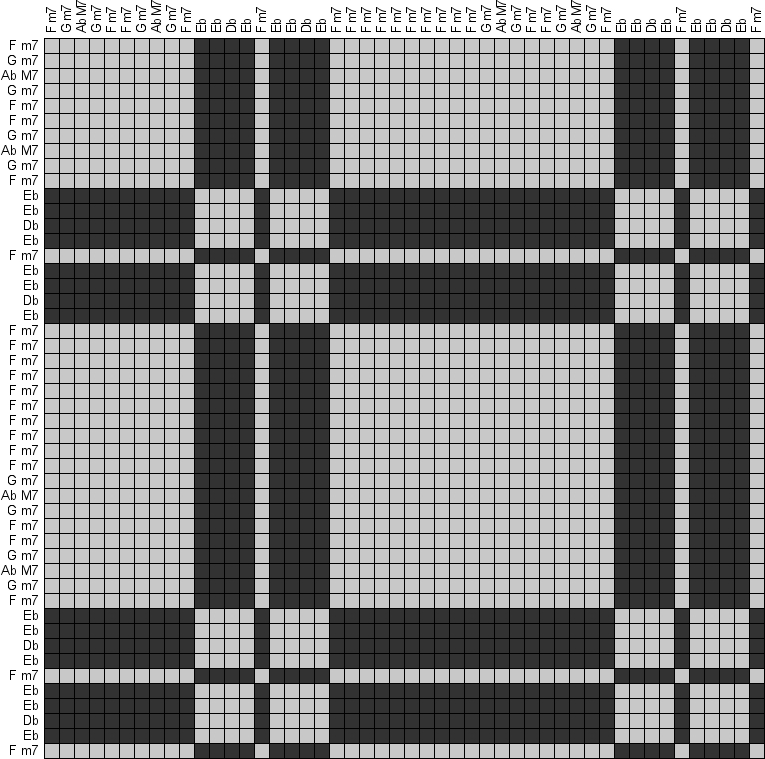
\includegraphics[width=3.5cm]{images/pretty3.jpg}\hspace{0.5cm}
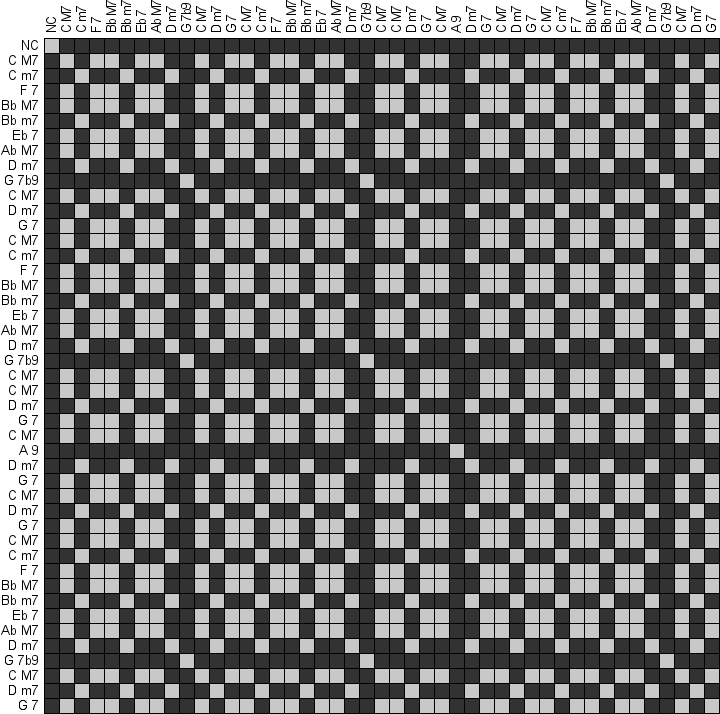
\includegraphics[width=3.5cm]{images/pretty4.jpg}
\caption{Several binary matrices revealing geometrical structure\label{pretty}}
\end{figure}

My first other idea was to compute a segmentation of the piece using the matrix (segmentation is a common way to analyse a music piece, since it gives a global structure). One can often see what looks like a partition of the matrix and consequently of the piece. However, such partitions can appear for different measures, sometimes very different thresholds. They may not appear at all for some pieces, or look very different. So I did not manage to design a satisfying algorithmical way to segment any piece.

The second way that I have been much interested in is \emph{grammatical inference} (or \emph{grammar induction}). As presented in \cite{goldabdallah}, formal grammars, that have been introduced for the modelling of spoken languages, have a lot of applications in Computer music. Furthermore, a grammar that could generate a piece or a corpus provides both a synthetic analysis and a way of creating similar pieces.

The problem of grammatical inference is, given two sets $S^+$ and $S^-$ (possibly empty) of words on a alphabet $\Sigma$ to compute a grammar of a certain form (regular grammar, context-free grammar\dots) that generates every word of $S^+$ but none of $S^-$. I have read many articles on the topic. For anyone who would be interested in it, \cite{bibliogrammar} is a good bibliographical introduction, and \cite{survey1} and \cite{survey2} a much complete introduction to state-of-the-art techniques. Several works use grammatical inference on a very close topic to mine: finding a structure inside jazz chords (not like me for a sequence of chords, but for the different chords used in jazz among all the possible combinations of notes) : \cite{jazzgrammar1}, \cite{jazzgrammar2}, \cite{jazzgrammar3}, \cite{jazzgrammar4}.

Nevertheless, I did not find a way of combining my work with those techniques.

In conclusion, I consider that what I did provides an interesting analysis of the data I was given, but that it also reveals potentialities still untapped.


\subsection{Improving the compression scheme}

There would be many ways to improve the compression and especially the diagonal compression. Beyond those I already mentioned, I can imagine two important new ones.

The first would be to use as well informations from the melodies in complement of the chord sequences. There are of course many ways of combining them, and many papers about it. And it would be possible to do so since most of the songs from the database I worked on also contain informations about the melody.

The second would be to incorporate the works described in \cite{aucouturier2002finding}. This papers looks for diagonal patterns (from an audio input), but uses techniques from the field of image analysis (like blurring, convolutions, Hough transform\dots) to identify more sequences as diagonal patterns, even is they are slight holes, or a different orientation (see figure \ref{aucouturier}). I believe this could improve much the results of the algorithm I used.

\begin{figure}
\centering
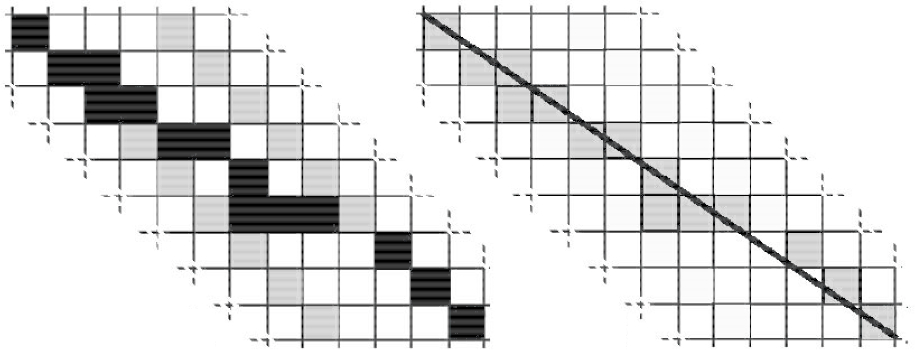
\includegraphics[width=7cm]{images/aucouturier.jpg}
\caption{An \guill{approximate diagonal pattern} (figure from \cite{aucouturier2002finding}) \label{aucouturier}}
\end{figure}

\subsection{The Lr2Cr8 project}

The Lr2Cr8 project\footnote{~~See \cite{Lrn2Cre8} for more information.} is a European project between six research institutes working on Computer music (Aalborg University being one of them). Its purpose is to develop \emph{learning} techniques of music in order to be able to \emph{create} new pieces. One way consists in adapting to composition already existing analysis methods.

In this context, I discussed with Olivier \textsc{Lartillot}, Ph. D. at Aalborg University, who worked in the same group as I did, about the adaptation of his tool, \textsc{PatMinr} (\cite{patminr}).
While I was trying to use grammatical inference in my own work, it appeared to me that a technique could be combined with his. Described in \cite{bracket2} and used in \cite{bracket1}, it is designed to infer grammar for a specific data, that has been bracketed beforehand so as to empathize its structure. Originally, this aimed at analysing natural languages, a bracketed data being for instance the sentence \guill{[My neighbour [ate [his yoghurt] [with [a spoon]]]]}.

It made me think of \textsc{PatMinr}, because the resulting decomposition of the melody it performs (figure \ref{bracket}, on the left) can easily be transformed into a bracketing (figure \ref{bracket}, on the right; colors are used for visibility but have no meaning). The challenging task, now, is to label cleverly the bracketed song, before applying the grammar induction methods. This idea is still currently being investigated.

\begin{figure}[h]
\centering
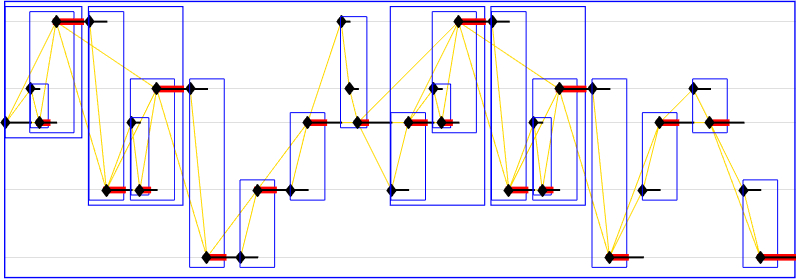
\includegraphics[width=7cm]{images/patminr1.jpg}\hspace{1cm}
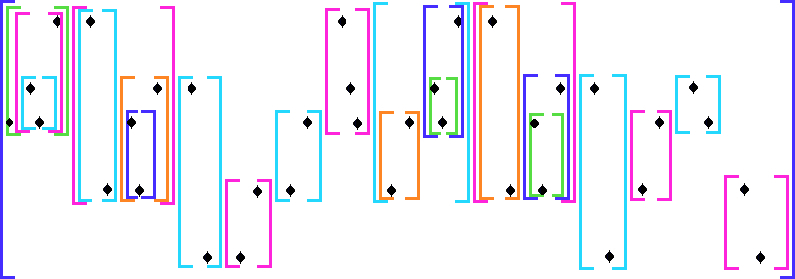
\includegraphics[width=7cm]{images/patminr2.jpg}
\caption{Analysis of a piece with \textsc{PatMinr} and resulting bracketing\label{bracket}}
\end{figure}


\section{Conclusion}

I have proposed two compression schemes for jazz chord sequences, which perform an interesting analysis of the data I had to study. They combine algorithms for compression without loss and similarity measures loosening the data. The global approach achieves better results than the linear one, showing general structure in jazz.

Moreover, this work brings forward the use of association measures for compression, which can be extended to many others analysis of chords; it asserts the usefulness of the F1-score in this context; and the binary matrices generated with these measures still show important potential for further investigations.

\newpage
\section{Bibliography}

\bibliographystyle{plain}
\bibliography{mabiblio}




\end{document}


